\chapter{Telemanipulátor geometria tervezése}
\label{sec:geometria}

Az általam tervezett telemanipulátor egyesíti mindazt, amit a teljes képzés során elsajátítottam. 

%----------------------------------------------------------------------------
\section{Geometria kialakítása}
%----------------------------------------------------------------------------

\begin{figure}[!ht]
\centering
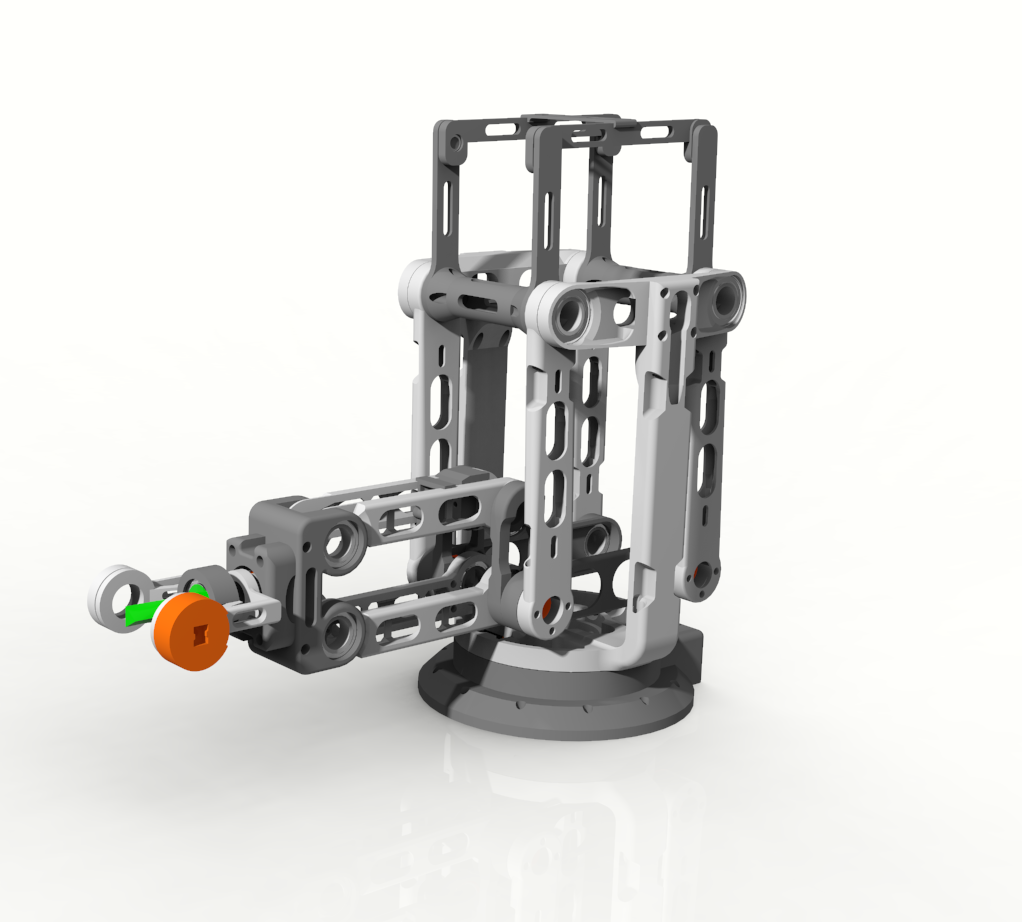
\includegraphics[width=120mm, keepaspectratio]{figures/Diploma_CAD/creo1.png}
\caption{Telemnanipulátor}
\label{fig:Telemnanipulátor}
\end{figure}

\begin{figure}[!ht]
\centering
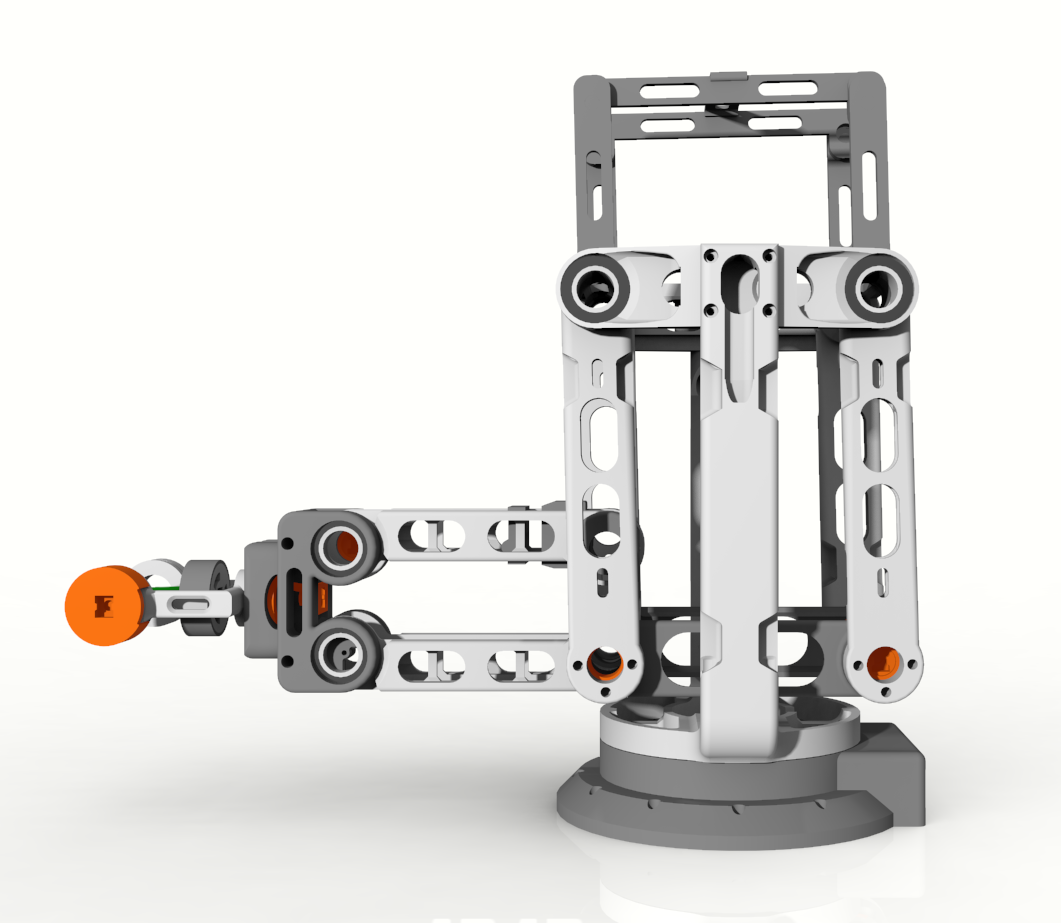
\includegraphics[width=120mm, keepaspectratio]{figures/Diploma_CAD/creo2.png}
\caption{Telemnanipulátor oldalról}
\label{fig:Telemnanipulátor}
\end{figure}


\begin{figure}[!ht]
\centering
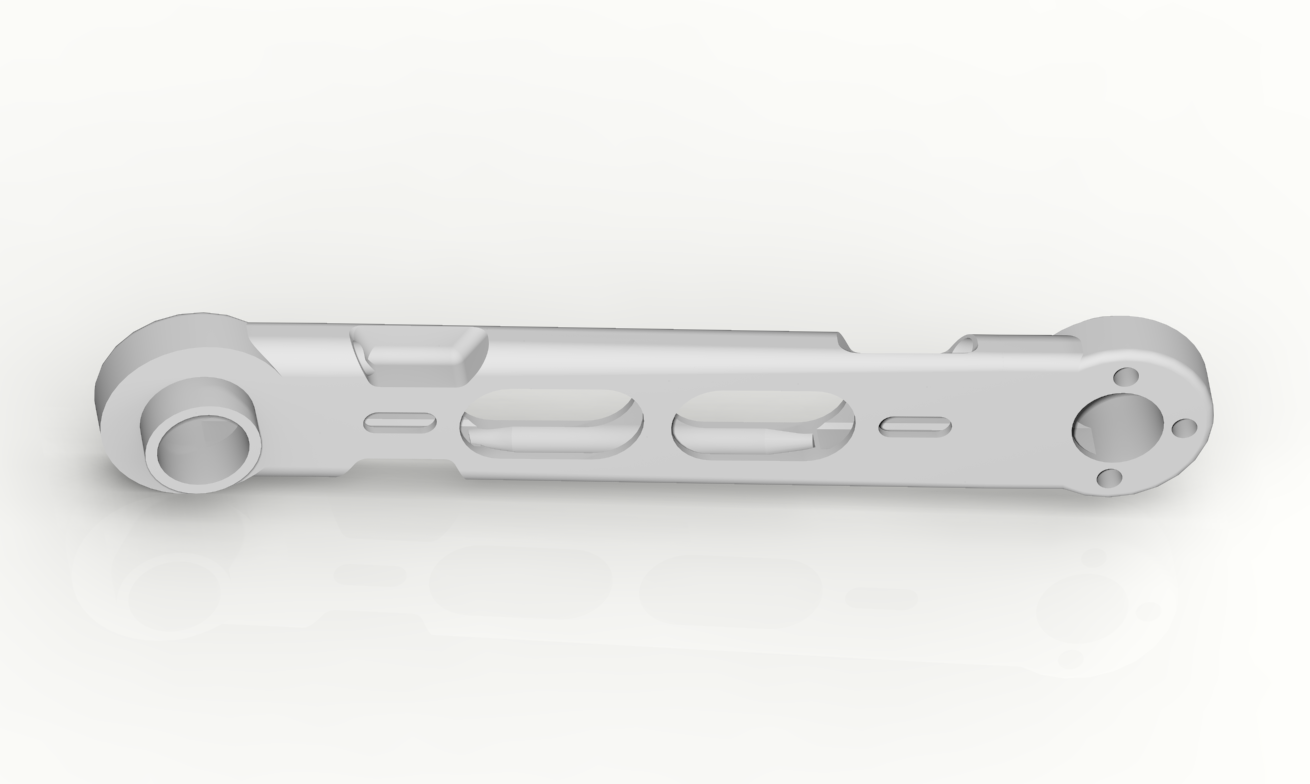
\includegraphics[width=150mm, keepaspectratio]{figures/Diploma_CAD/creo3.png}
\caption{Kar}
\label{fig:kar}
\end{figure}


\begin{figure}[!ht]
\centering
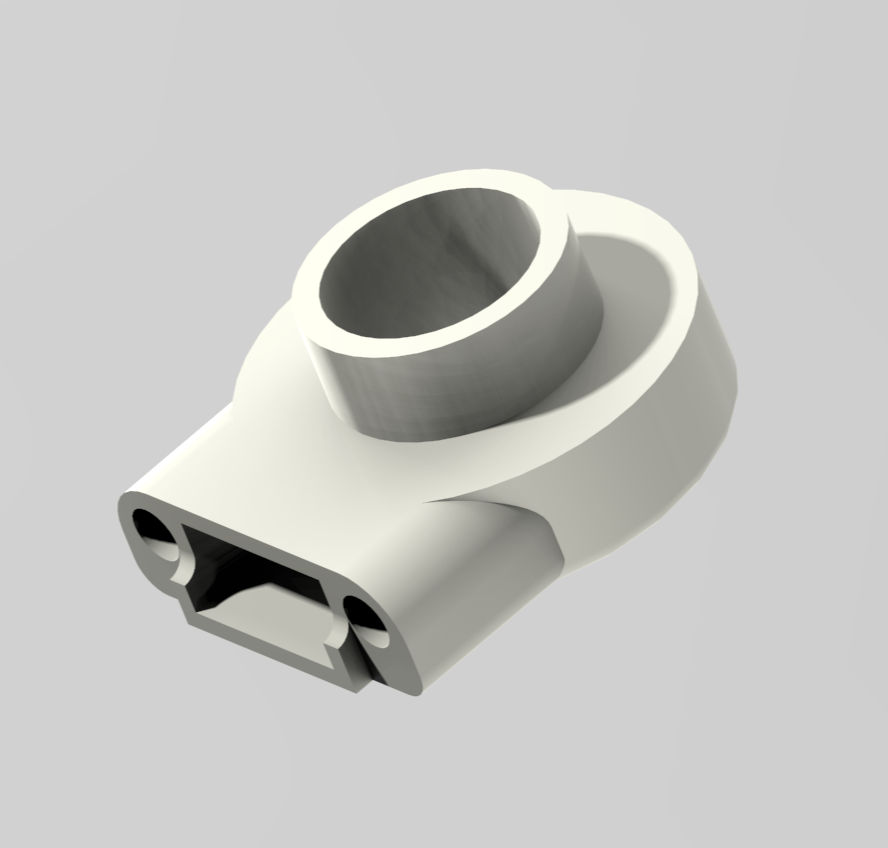
\includegraphics[width=70mm, keepaspectratio]{figures/Diploma_CAD/creo4.png}
\caption{Csuklo}
\label{fig:Csuklo}
\end{figure}


\section{Kinematikai modell felépítése}

\begin{figure}[!ht]
\centering
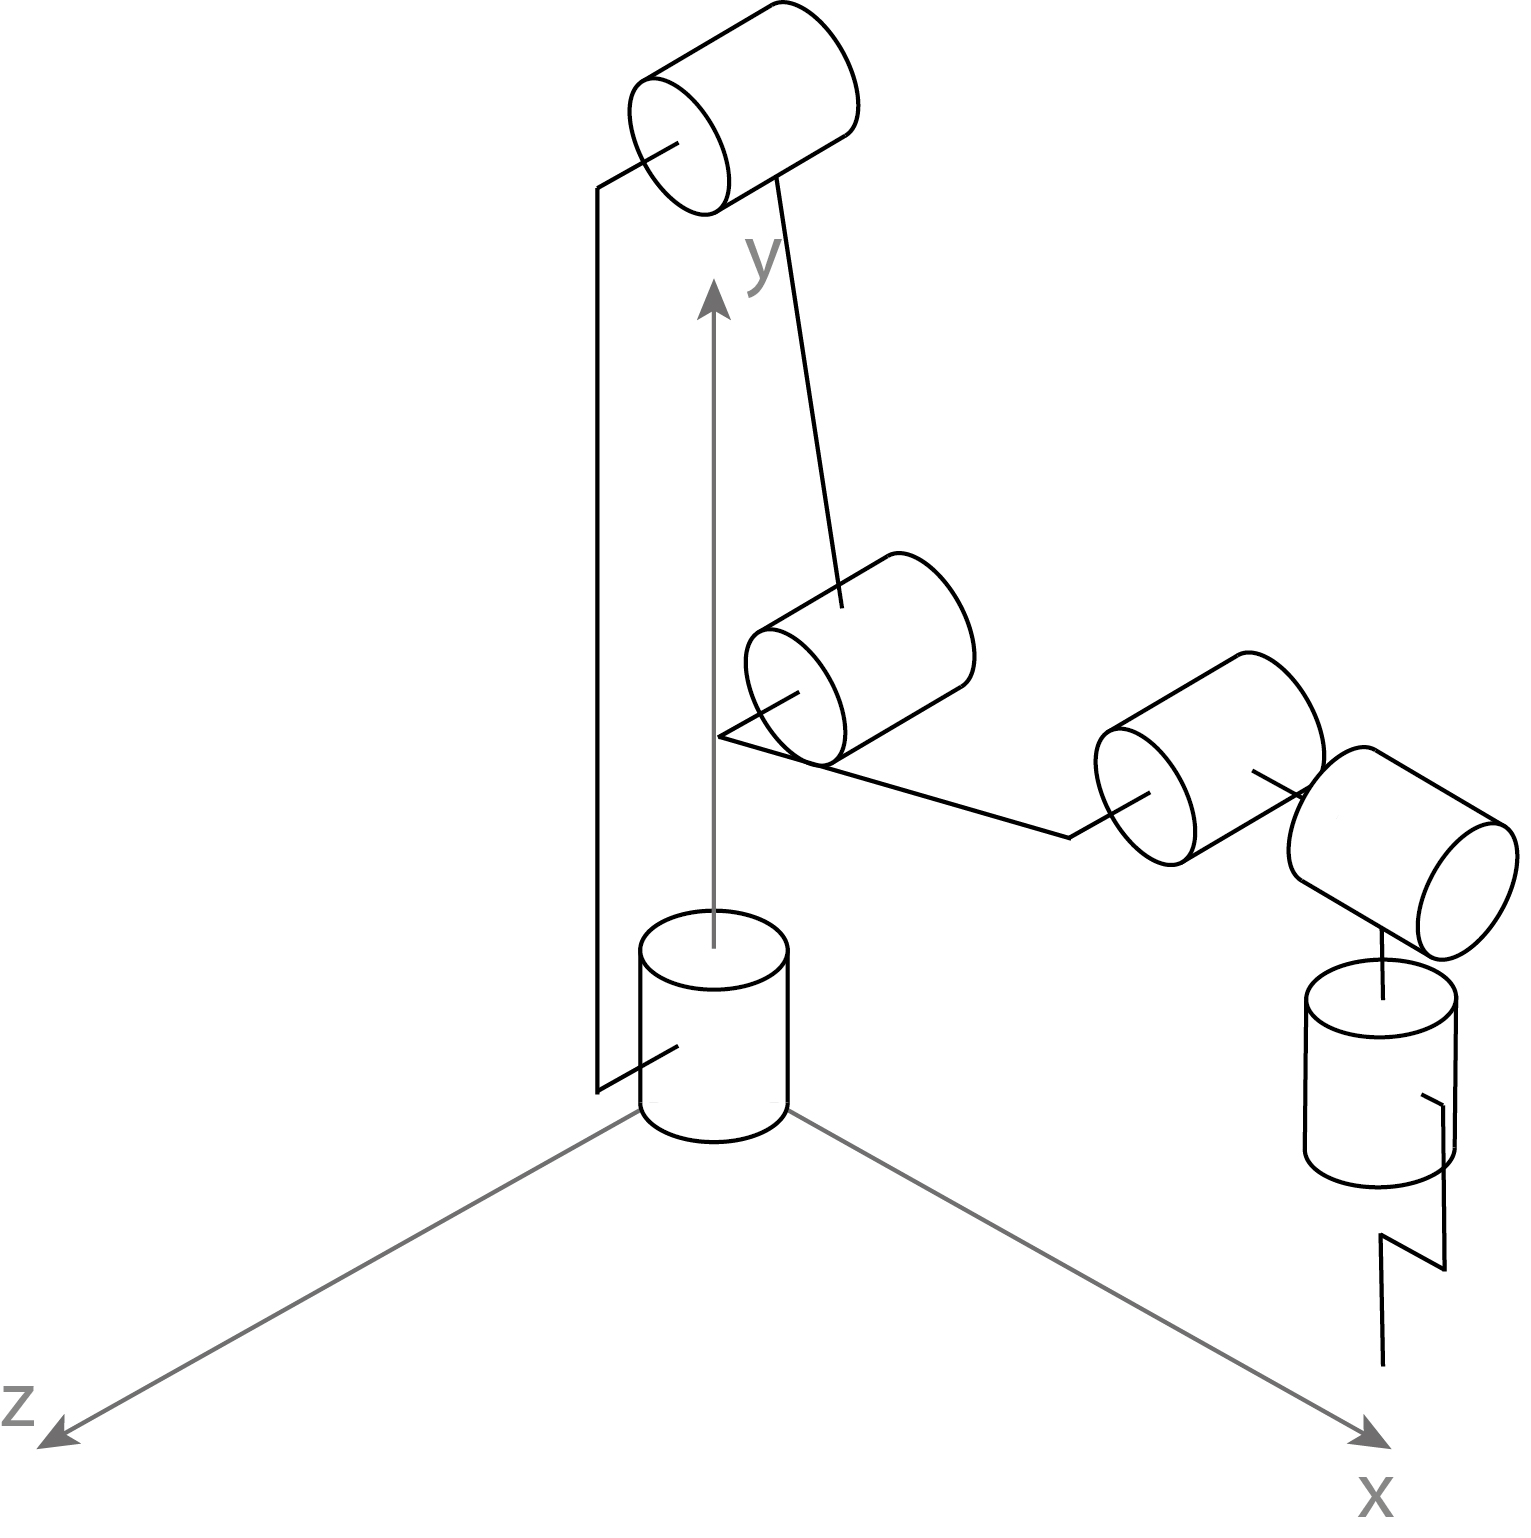
\includegraphics[width=70mm, keepaspectratio]{figures/Szakdoga/kinematik_v_2}
\caption{Szakdolgozat kinematika}
\label{fig:Csuklo}
\end{figure}

\begin{figure}[!ht]
\centering
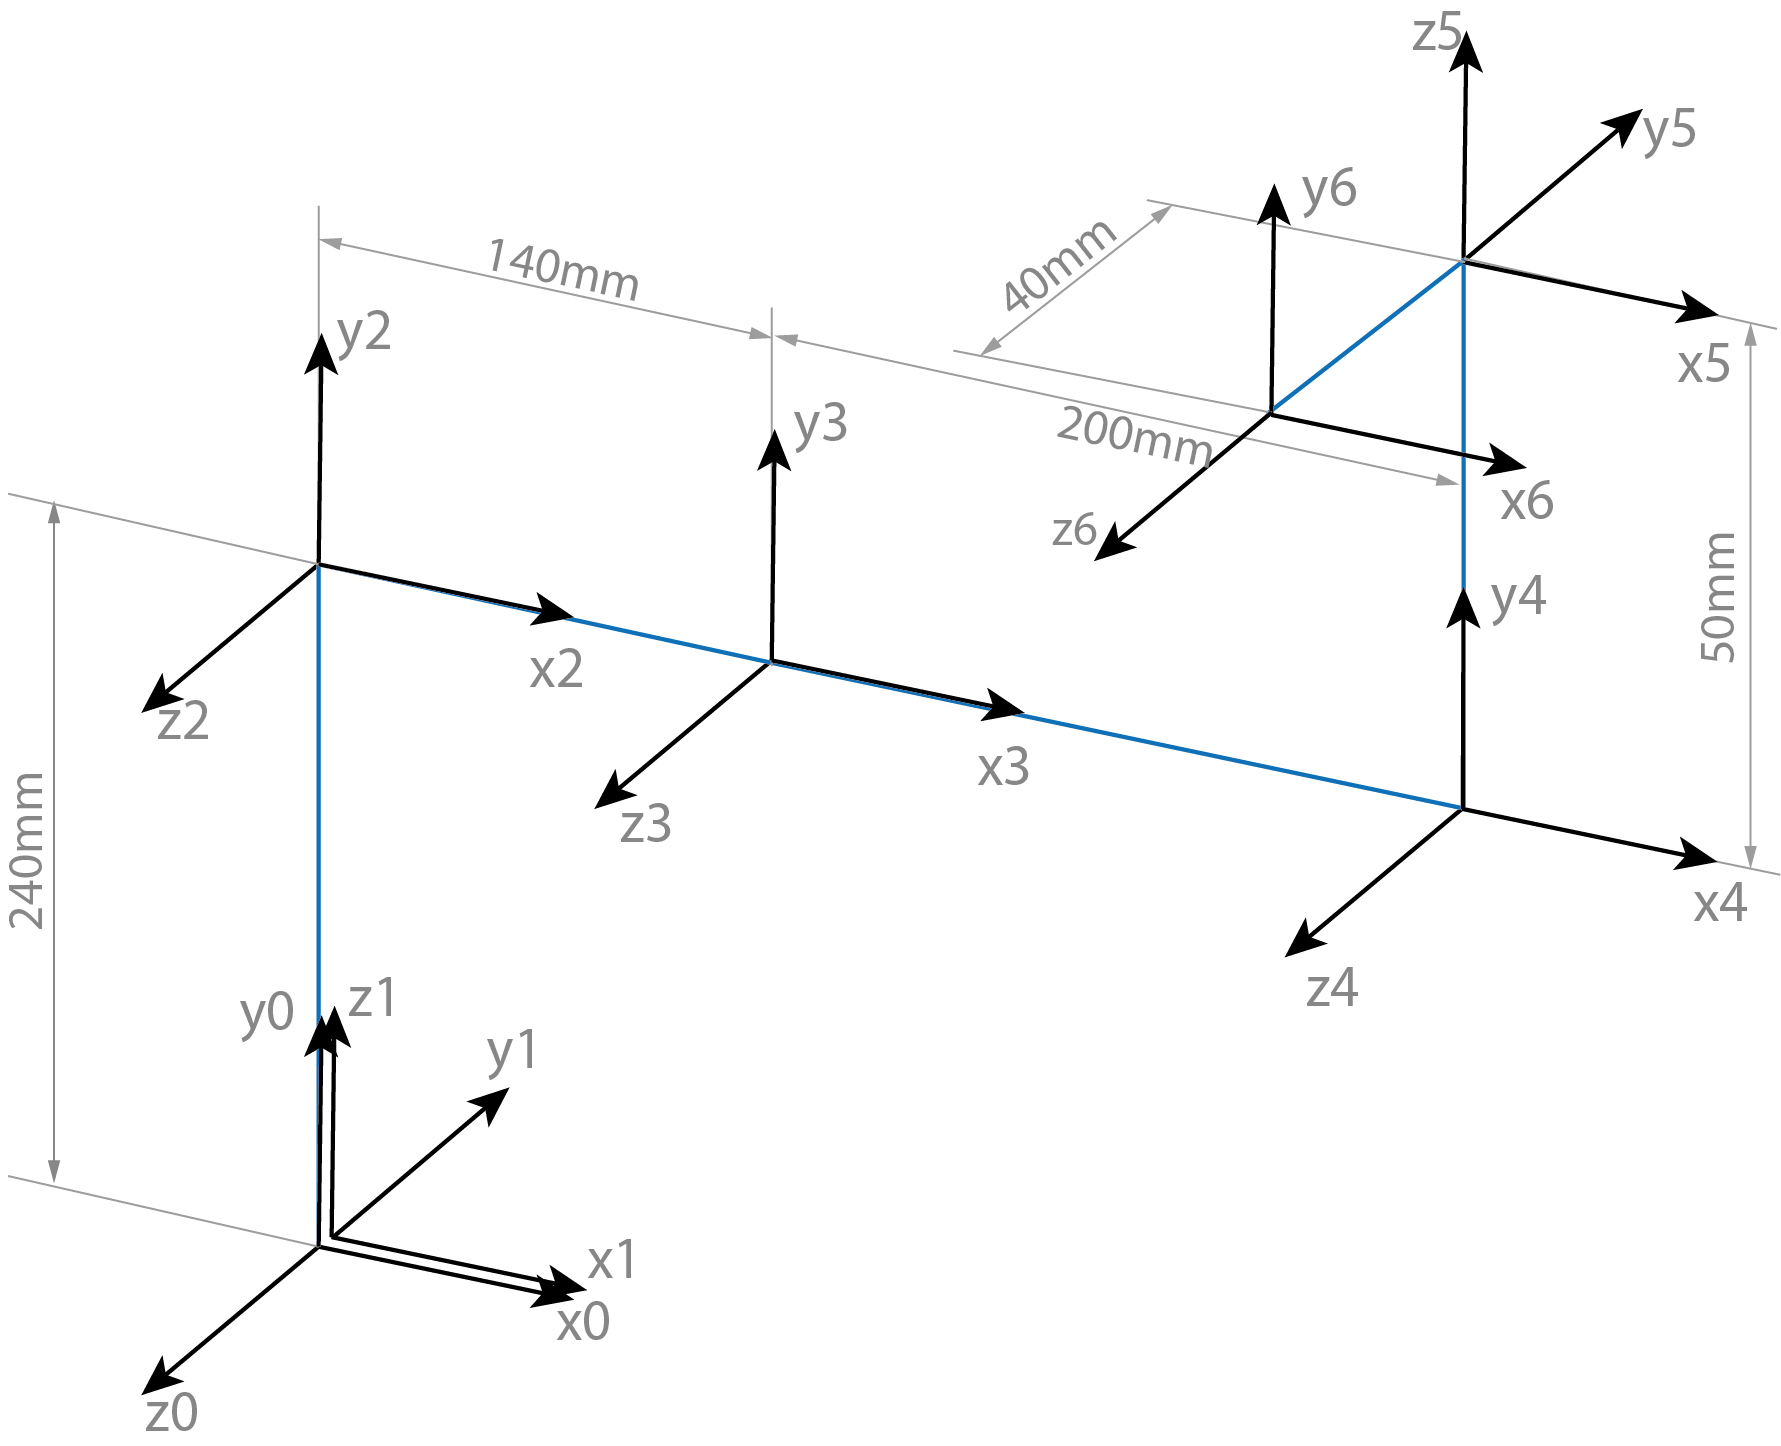
\includegraphics[width=70mm, keepaspectratio]{figures/Szakdoga/v_2_dh}
\caption{Szakdolgozat Denavit-Hartenberg felírás}
\label{fig:Csuklo}
\end{figure}

\begin{figure}[!ht]
\centering
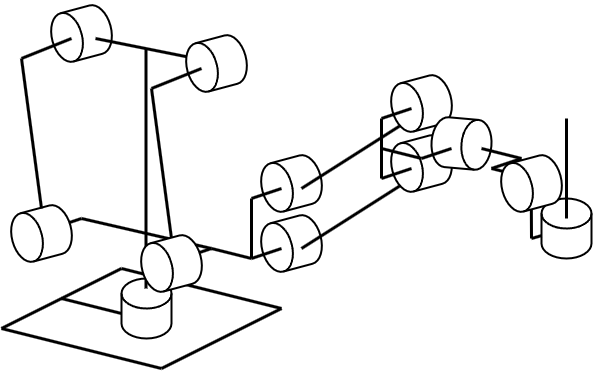
\includegraphics[width=70mm, keepaspectratio]{figures/Diagrammok/Diploma_kinematika}
\caption{Diploma munka kinematika}
\label{fig:Csuklo}
\end{figure}


\begin{figure}[!ht]
\centering
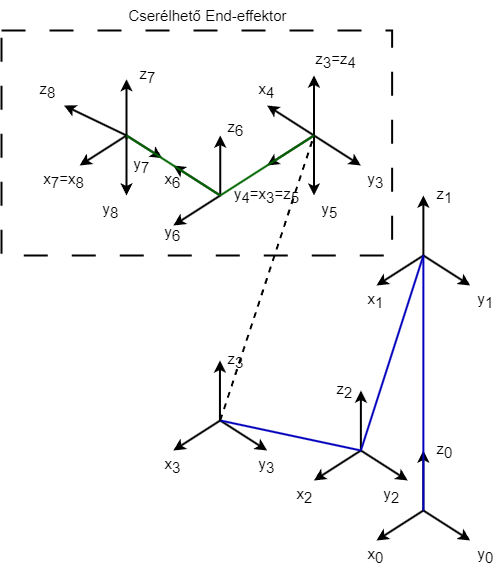
\includegraphics[width=70mm, keepaspectratio]{figures/Diagrammok/DH_feliras}
\caption{Diploma munka Denavit-Hartenberg felírás}
\label{fig:Csuklo}
\end{figure}



\subsection{Direkt kinematika}
%----------------------------------------------------------------------------
A direkt kinematika és a Khali-féle Denavit-Hartenberg (DH) módszer a robotika területén alkalmazott módszerek, amelyek lehetővé teszik a robotkarok és manipulátorok mozgásterének és pozíciójának meghatározását. Az alábbiakban bemutatom ezeket a módszereket és azok fő jellemzőit.

A direkt kinematika a robotkarok mozgásterének és végpontjainak pozíciójának meghatározását vizsgálja. Célja, hogy a robotkar ízületeinek állapotából vagy koordináta rendszeréből kiindulva meghatározza a végpont vagy a szerszám pozícióját a világkoordináta rendszerben. Ez a módszer matematikai modelleket és transzformációkat használ a kar szegmenseinek és ízületeinek geometriájának leírására és kapcsolatának meghatározására.

A Khali-féle DH módszer a direkt kinematika egyik legelterjedtebb módszere, amelyet a Denavit-Hartenberg (DH) paraméterek felhasználásával végeznek. Ez a módszer egy koordináta rendszer hierarchikus láncolását használja a robotkar szegmensei közötti kapcsolat leírására. A DH módszerben a kar szegmenseinek geometriáját és relatív helyzetét négy paraméter segítségével írják le: az alfa, a, d és theta paraméterek.

Az alfa paraméter az aktuális ízület tengelyének elfordulását jelenti a szomszédos szegmens tengelyéhez képest. Az a paraméter a szegmens hosszát vagy az ízület távolságát jelenti az előző szegmenstől. A d paraméter a szegmens központjának távolságát jelenti az előző szegmenstől a közös tengely mentén. A theta paraméter pedig az aktuális ízület elfordulását jelenti.

A DH módszerben minden szegmenst leíró paramétert és transzformációs mátrixot alkalmaznak, amelyek segítségével a végpont pozícióját határozzák meg. A módszer iteratív módon alkalmazható, a végponttól visszafelé haladva az egyes ízületek állapotának és pozíciójának meghatározására.

A direkt kinematika és a DH módszer széles körben alkalmazott eszközök a robotika területén. Segítségükkel lehetőség nyílik a robotkarok mozgásának tervezésére, szimulációjára és vezérlésére. Ezen módszerek alkalmazásával pontosan meghatározható a robotkar végpontjának helyzete és orientációja a világkoordináta rendszerben, ami fontos információ lehet a munkafolyamatok tervezésében és végrehajtásában.

Összességében a direkt kinematika és a Khali-féle DH módszer lehetővé teszik a robotkarok mozgásterének és pozíciójának meghatározását. Ezek a módszerek alapvetőek a robotika területén, és fontos szerepet játszanak a robotkarok tervezésében, szimulációjában és vezérlésében. A direkt kinematika és a DH módszer segítségével precízen modellezhetők és kontrollálhatók a robotkarok mozgásai, amelyek számos ipari és egyéb alkalmazásban hasznosak lehetnek.

\subsection{Inverz kinematika}
%----------------------------------------------------------------------------
Az inverz kinematika a robotika területén használt módszer, amely lehetővé teszi a robotkarok számára, hogy meghatározzák az ízületeik állapotát és pozícióját a kívánt végpont vagy TCP (tool center point) eléréséhez. Ez a módszer a direkt kinematika ellentéte, mivel itt nem a végpont pozícióját kell meghatározni az ízületek ismert állapota alapján, hanem éppen fordítva: az ízületek állapotát kell meghatározni a kívánt végpont pozíciója alapján.

Az inverz kinematika alkalmazása során a robotkar rendszerének geometriáját és ízületeinek korlátait figyelembe véve meg kell határozni az ízületek szögét vagy állapotát, amelyekkel a TCP a kívánt pozícióba kerül. Ez egy matematikai probléma, amelyet általában numerikus vagy analitikus megoldó algoritmusok segítségével oldanak meg.

Az inverz kinematika számos alkalmazási területtel rendelkezik a robotikában. Például a gyártósorokon, ahol a robotkaroknak pontosan kell pozícionálniuk a szerszámokat vagy alkatrészeket, az inverz kinematika segítségével a kívánt végpont pozíció alapján meg lehet határozni az ízületek állapotát. Ez lehetővé teszi a robotkarok pontos és ismételhető mozgását a gyártási feladatok hatékony végrehajtása érdekében.

A Khali-féle DH módszer a robotkarok leírására és az inverz kinematika alkalmazására is használt módszer. Ennek során a robotkar ízületeinek és szegmenseinek geometriáját és kapcsolatát a Denavit-Hartenberg (DH) paraméterek segítségével írják le. Ezek a paraméterek az alfa, a, d és theta értékekből állnak, amelyek meghatározzák az ízületek elfordulását és a szegmensek geometriáját.

A DH paraméterekkel leírt robotkar geometriáját felhasználva a Khali-féle DH módszerrel meghatározható az inverz kinematika. Az algoritmus segítségével a kívánt végpont vagy TCP pozíciója alapján a szükséges ízületi szög vagy állapot meghatározható. Az így kapott eredményeket a robotvezérlő egység továbbítja a robotkar motorjainak, hogy a megfelelő pozícióba mozgassa a TCP-t.

Az inverz kinematika és a Khali-féle DH módszer együttműködve lehetővé teszik a robotkarok számára, hogy a kívánt végpont vagy TCP pozíciókba helyezkedjenek el. Ez kulcsfontosságú a precíz munkavégzéshez és a különböző feladatok hatékony végrehajtásához a robotika számos alkalmazási területén, például az ipari automatizációban, a gyártásban, a logisztikában és a sebészeti beavatkozásokban. Az inverz kinematika és a Khali-féle DH módszer jelentős fejlődést hozott a robotkarok irányításában és pozícionálásában, és további lehetőségeket teremt a robotika területén.